\usetikzlibrary{shapes}
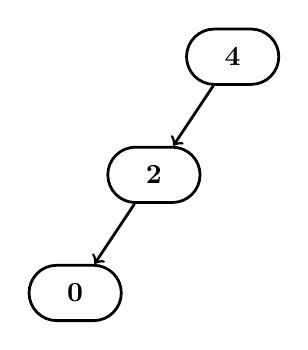
\begin{tikzpicture}[line width=1pt]
\tikzstyle{con}=[draw,font=\bfseries,rounded rectangle,minimum height=2em,minimum width=4em];
\tikzstyle{dir}=[->];

\node [con] (v2) at (-0.5,1) {2};
\node [con] (v3) at (-1.5,-0.5) {0};
\node [con] (v1) at (0.5,2.5) {4};
\draw [dir] (v1) edge (v2);
\draw [dir] (v2) edge (v3);
\end{tikzpicture}